\setcounter{chapter}{4}
\chapter{Cinématique}
\section{Généralités}

Le mot cinématique vient du grec kinema qui signifie mouvement. La cinématique étudie les mouvements \trou{indépendamment} de leurs causes à savoir les forces.

\subsection{Nécessité de définir un \trou{référentiel}}

Critiquez la formulation de la question: "Êtes-vous immobile ou en mouvement ?" \\

\trou{Nous sommes immobile par rapport au sol et en mouvement par rapport au Soleil. Il est donc indispensable de définir un solide de référence: un référentiel.}

\blocrouge{Définition}{\trou{Un référentiel est un solide considéré immobile par rapport auquel on étudie le mouvement d'un système.}}

L'objet dont on étudie le mouvement est appelé le \textbf{système}. En général, on étudie un point de ce système, le plus souvent il s'agit du centre de gravité.
\subsection{Trajectoire et Chronophotographie}

\blocrouge{Définition}{L'ensemble des positions successives occupées par un point mobile M au cours du temps s'appelle la trajectoire.\\ En relevant à intervalle de temps régulier, la position du point mobile, on obtient une chronophotographie.}

\etiquette{Exemples}
Représentez l'allure de la chronophotographie dans les cas suivants:
\begin{enumerate}
	\item Une bille que l'on lâche
	\item Une bille en mouvement rectiligne uniforme roulant sur le sol (parfaitement glissant).
	\item Un ballon de basket lors dans lancer franc.
	\item Un point en mouvement circulaire uniforme.
\end{enumerate}
\vspace{6 cm}


\section{Le vecteur vitesse}
Le nombre est bien adapté à la description de certaines grandeurs physiques comme la distance, la température, la concentration molaire... Cependant il n'est pas adapté pour décrire un déplacement, une vitesse ou encore une accélération. 
\subsection{Construction à partir d'une chronophotographie}

Faire les questions 1 et 2 du problème à 1D et du problème à 2D sur la fiche pratique "Comment Exploiter une Chronophotographie"

	\subsection{Projections et coordonnées cartésiennes}
	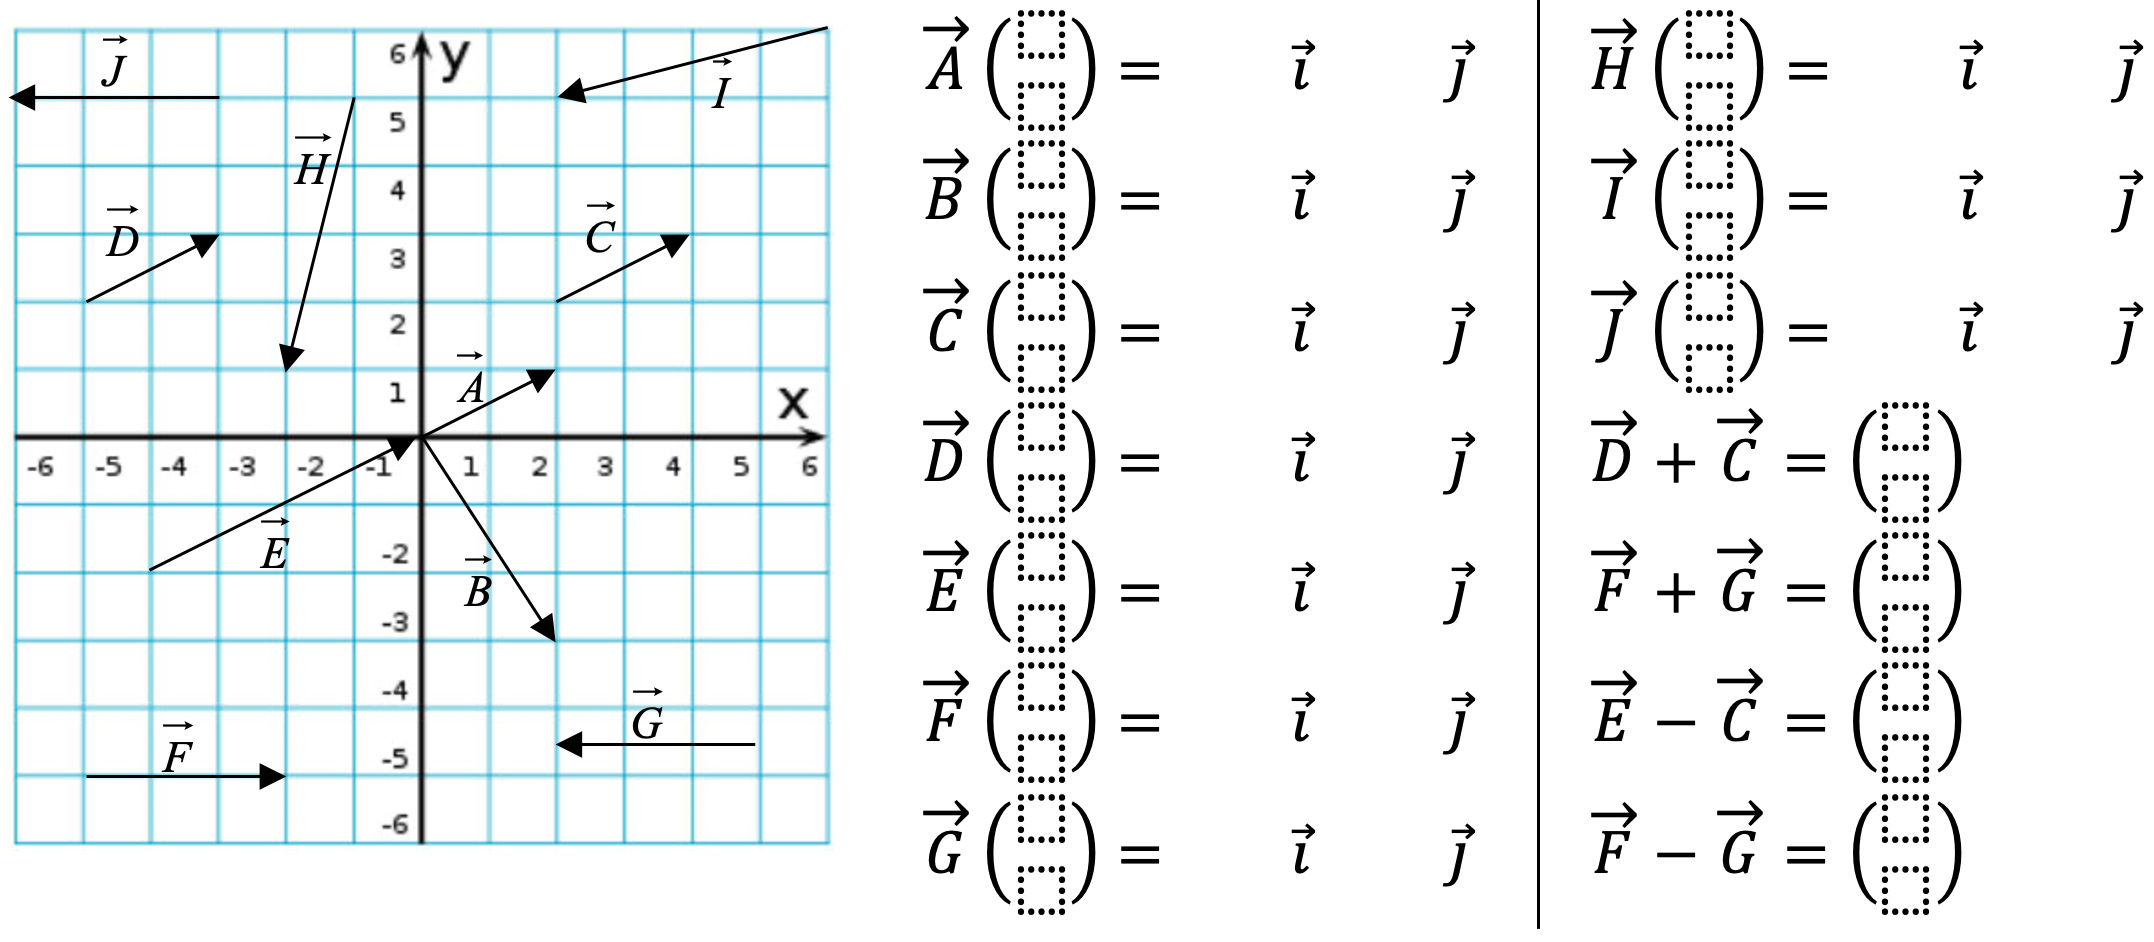
\includegraphics[height=6cm]{figures/cinematique_1}\\
		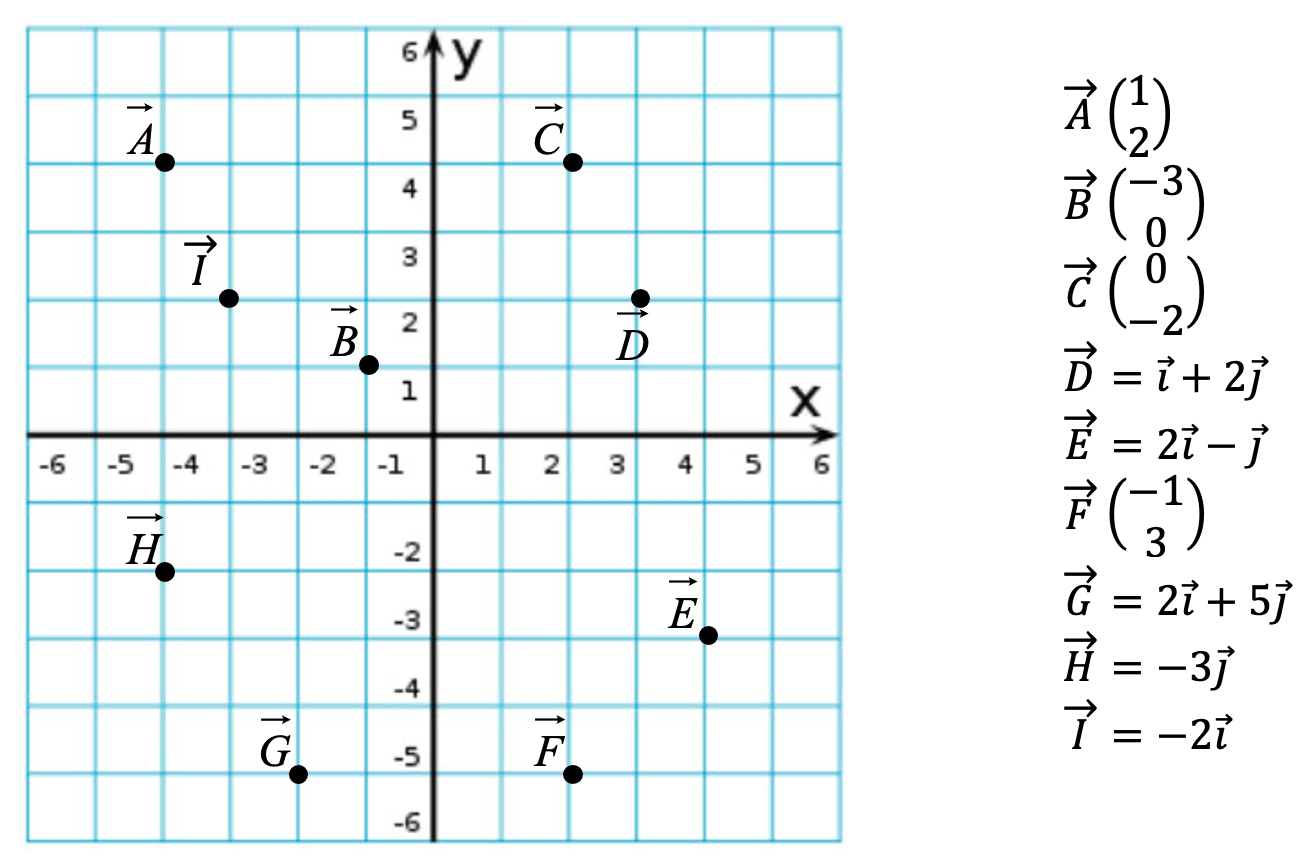
\includegraphics[height=6cm]{figures/cinematique_2}
	\subsection{Position et Vecteur position}
	
Le point M est en mouvement, sa position dépend du temps. C'est pourquoi dans la suite les coordonnées de M sont des fonctions du temps. \\On les note: $x(t)$, $y(t)$ et $z(t)$

Le vecteur position est le vecteur qui relie l'origine du repère et le point mobile M. Il se note: $\overrightarrow{OM(t)}$ ses coordonnées sont les même que le point M. 

\blocrouge{A retenir}{\\
\begin{minipage}{.3\textwidth}
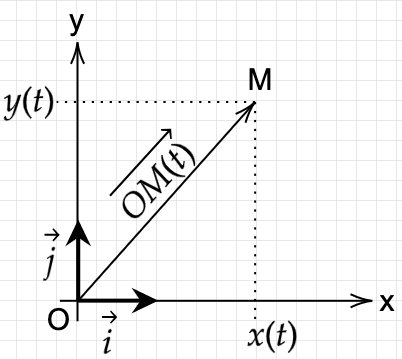
\includegraphics[scale=0.33]{figures/cinematique_3.png}	
\end{minipage}
\hfill
\begin{minipage}{.65\textwidth}
Le vecteur position $\overrightarrow{OM(t)}$  a pour coordonnées: \trou{$
\begin{pmatrix}
	x(t) \\ y(t)
\end{pmatrix}
$}
\\


Une autre écriture est: $\overrightarrow{OM(t)}=$ \trou{$x(t). \vec{i}+y(t). \vec{j}$}
\end{minipage}
}


\paragraph*{Remarques} L'unité de chaque coordonnées est le mètre (m). \\A l'instant initial t=0s, l'abscisse x se notera $x(t=0)$ ou $x(0)$.

\subsection{Dérivation en Math vs Dérivation en Physique}

\etiquette{En math}
En mathématique, on note $f'(x)$ la fonction dérivée de $f(x)$. 
\\ Si $f(x)= 10x^2 -2x + 1$ Alors $f'(x) = 10\times 2.x - 2 + 0 = 20x -2$ 
\\
\etiquette{En Physique}

Au lieu de $f'(x)$ on écrira $\frac{df(x)}{dx}$ ou encore $\frac{df}{dx}$ si il est évident que la variable est $x$.  Donc $$\frac{df}{dx} = 20.x -2$$


Dans ce chapitre, la variable est le temps $t$. Considérons une fonction $g$ de la variable $t$ qui s'écrit: 

\begin{align*}
	g(t) &= -3t^2 + 4t +8\\
	g'(t) &= \trou{- 6t + 4 }\\
	\frac{dg}{dt} &= \trou{-6t+4}
\end{align*}

\etiquette{Exercice}
En cinématique,  on dispose  d'une fonction $x(t) = -\frac{1}{2}t^2 + 3t -7$. Calculer $\frac{dx}{dt}$.

\trou{$frac{dx}{dt}=-t+3$}.


\etiquetterouge{Attention}

Ne pas confondre le $x$ des maths avec le $x(t)$ de la physique !
\newpage
\subsection{Vitesse instantanée et vecteur vitesse}

Vitesse est une expression vague. Il faut parler de \trou{vecteur vitesse} ou bien de \trou{valeur de la vitesse}.

La valeur de la vitesse à un instant précis $t$ s'écrit $v(t)$ et s'exprime en m/s. C'est donc la valeur de la vitesse à la date t.
\\

\blocrouge{Vecteur vitesse $\overrightarrow{v(t)}$ }{\\
\begin{minipage}{.5\textwidth}
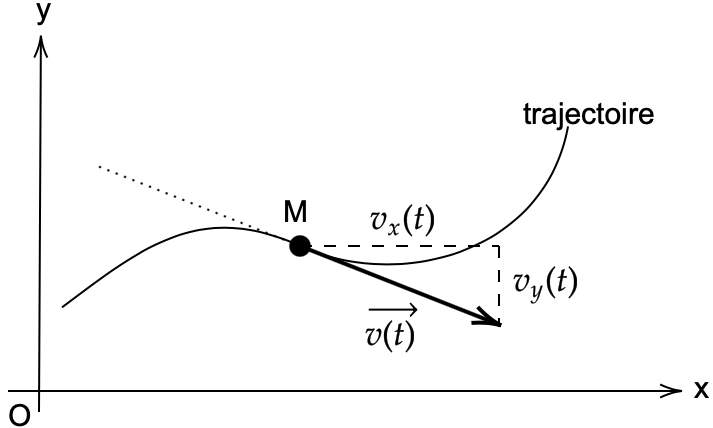
\includegraphics[scale=0.30]{figures/cinematique_4.png}	
\end{minipage}
\hfill
\begin{minipage}{.45\textwidth}
Caractéristiques:
\begin{itemize}
	\item  Direction: Tangente à la trajectoire
	\item Sens: Celui du mouvement
	\item Valeur: la valeur de la vitesse $v(t)$
\end{itemize}
	
\end{minipage}
}


\blocrouge{Définition mathématique du vecteur vitesse}{$$\overrightarrow{v(t)}=\frac{d\overrightarrow{OM(t)}}{dt}$$


Cela signifie que les coordonnées de $\overrightarrow{v(t)}$ s'obtiennent en dérivant les coordonnées  $x(t)$ et $y(t)$ du vecteur position $\overrightarrow{OM(t)}$.

Les coordonnées de $\overrightarrow{v(t)}$ s'écrivent: 


 \[
 \overrightarrow{v(t)} 
\begin{pmatrix}
	v_x(t) = \frac{dx(t)}{dt} \\
		v_y(t) = \frac{dy(t)}{dt}
\end{pmatrix}
\]

}




Pour calculer, les coordonnées de $\vec{v}$ il faudra dériver par rapport au temps les fonctions $x(t)$ $y(t)$ et $x(t)$. 


\subsection{Du vecteur $\vec{v}$ à sa valeur $v$}

\etiquetterouge{Erreur à éviter !}
Il ne faut pas croire qu'un vecteur est un nombre ! Ainsi $\vec{v}$ n'est pas égal à un nombre de m/s.
\\On peut cependant écrire: $$\vec{v}=v_x(t).\vec{i}+v_y(t).\vec{j}$$ il y a bien des vecteurs à gauche est à droite du signe $=$.

La valeur du vecteur $\overrightarrow{v(t)}$ qui s'écrit $v(t)$  est la vitesse instantanée en m/s. Cette valeur s'obtient à partir des coordonnées de $\overrightarrow{v(t)}$.



\blocrouge{Valeur de la vitesse instantanée}{Soit le vecteur vitesse $\overrightarrow{v(t)}$ de coordonnées $v_x(t)$ et $v_y(t)$. La valeur de la vitesse $v(t)$ en m/s vaut:$$v(t)=\trou{\sqrt{v_x(t)^2+v_y(t)^2}}$$

La valeur de la vitesse est aussi appelée norme du vecteur vitesse.
}

\etiquette{Application}

Répondre aux questions de 1 à 7 de la partie Trajectoire et vecteur vitesse de la fiche "Exploiter des équations horaires"

\section{Le vecteur accélération}
\subsection{Construction du vecteur accélération à partir d'une chronophotographie}

\etiquette{Exercice}

Faire la partie Construction du vecteur accélération du problème à 1D et à 2D de la fiche "Comment exploiter une chronophotographie"

\subsection{Calcul du vecteur accélération}
\blocrouge{Définition mathématique du vecteur accélération}{$$\overrightarrow{a(t)}=\frac{d\overrightarrow{v(t)}}{dt}$$


Cela signifie que les coordonnées de $\overrightarrow{a(t)}$ s'obtiennent en dérivant les coordonnées  $v_x(t)$ et $v_y(t)$ du vecteur position $\overrightarrow{v(t)}$.

Les coordonnées de $\overrightarrow{a(t)}$ s'écrivent: 


 \[
 \overrightarrow{a(t)} 
\begin{pmatrix}
	a_x(t) = \trou{\frac{dv_x(t)}{dt}} \\
		a_y(t) = \trou{\frac{dv_y(t)}{dt}}
\end{pmatrix}
\]

}

\paragraph*{Remarques} 
	\begin{itemize}
		\item Le vecteur accélération n'est pas en général dans le sens du mouvement contrairement au vecteur vitesse qui l'est toujours.
		\item On peut obtenir les coordonnées de $\overrightarrow{a(t)}$ en dérivant deux fois les coordonnées de $\overrightarrow{OM(t)}$ Lire point math p 227.
	\end{itemize}

 \etiquetterouge{Erreur à éviter}

\begin{itemize}
\item Le vecteur accélération comme tous les vecteurs n'est JAMAIS égal à un nombre.
		\item Un vecteur accélération non nul ne signifie pas que la valeur de la vitesse augmente (ou diminue). Voir plus loin le cas du mouvement circulaire uniforme.

\end{itemize}
		
\subsection{Calcul de la valeur de l'accélération}
\blocrouge{Valeur de l'accélération }{Soit le vecteur accélération $\overrightarrow{a(t)}$ de coordonnées $a_x(t)$ et $a_y(t)$. La valeur de l'accélération $a(t)$ en mètre par seconde carré vaut:$$a(t)=\sqrt{a_x(t)^2+a_y(t)^2}$$
L'unité de $a(t)$ est: $m/s^2$ ou $m.s^{-2}$

}

\etiquette{Exercice}

Finir la fiche "Exploiter des équations horaires"


\section{Première Synthèse des résultats}
\etiquette{Propriétés des Mouvements Rectilignes à connaître}



\begin{tabular}{|l|l|l|l|}
\hline

  Mouvements&Description & Mathématiques & Exemples\\
\hline  \hline
MRU  & Trajectoire: Droite& $\vec{v}=\trou{\vec{v_0} = \overrightarrow{cste}}$& \trou{Palet de hockey}\\
& Vistesse constante & $\vec{a(t)}=\trou{\vec{0}}$&\\
\hline
MR & Trajectoire: Droite & $\vec{a(t)}=\vec{a_0}= \overrightarrow{cste}$& \trou{-Balle lancée vers le haut}\\
uniformément & $v$ peut augmenter & $\vec{v(t)}=\vec{a_0}\times t+\vec{v_0}\neq \overrightarrow{cste}$& \trou{(phase ascendante)}\\
accéléré & v peut diminuer& &\trou{- Chute libre}\\
\hline

\end{tabular}

\vspace{1cm}
\etiquette{Réactivation}

Pour chacun des exemples du tableau: 
\begin{enumerate}
	\item Représenter une chronophotographie du mouvement.
	\item Représenter quelques vecteurs vitesses de manière réaliste.
	\item Représenter quelques vecteurs accélérations de manière réaliste.
\end{enumerate}


\newpage
\section{Cas des mouvements circulaires}
Dans tout ce qui suit, M est en mouvement circulaire. Sa trajectoire est un cercle de centre O et de rayon R.
\subsection{Base de Frenet}
Pour décrire un mouvement circulaire, on utilise un autre repère: \textbf{la base de Frenet}.
L'utilisation de cette base permet de décrire simplement $\vec{v(t)}$ et $\vec{a(t)}$.

\etiquette{Description}

La base de Frenet a pour origine le point mobile M. De plus, elle possède 2 vecteurs unitaires: $\vec{u_t}$ et $\vec{u_n}$ (parfois aussi noté $\vec{T}$ et $\vec{N}$)
\begin{itemize}
	\item $\vec{u_t}$ est un vecteur  \trou{ tangent } au cercle dans le sens du mouvement de M. 
	\item $\vec{u_n}$ est un vecteur \trou{perpendiculaire} à $\vec{u_t}$ orienté vers l'intérieur du cercle
\end{itemize}

\subsection{Vecteurs dans la base de Frenet}
\blocrouge{Définitions}{


\begin{minipage}{.5\textwidth}
Dans la base de Frenet, pour un mouvement circulaire quelconque les vecteurs vitesse et accélération s'écrivent:
\\
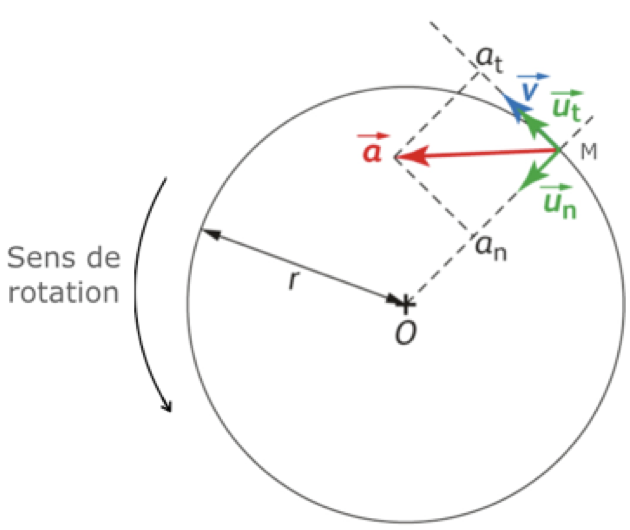
\includegraphics[scale=.65]{figures/cinematique_6}
\\	
\end{minipage}
\begin{minipage}{.45\textwidth}
	$$\vec{v(t)}= v(t). \vec{u_t}$$
		$$\vec{a(t)}= \frac{dv(t)}{dt}. \vec{u_t} + \frac{v^2(t)}{R}.\vec{u_n}$$
		Dans cette base, $\vec{a(t)}$ a pour coordonnées:
	 \[
 \overrightarrow{a(t)} 
\begin{pmatrix}
	a_t(t) = \trou{\frac{dv(t)}{dt}} \\
		a_n(t) = \trou{\frac{v^2(t)}{R}}
\end{pmatrix}
\]

\end{minipage}
}
\paragraph*{Remarque:} Les  vecteurs $\vec{u_t}$ et $\vec{u_n}$ représentés ci-dessus tournent comme M. La base de Frenet: $\vec{u_t}$ et $\vec{u_n}$ est mobile contrairement à la base en coordonnées cartésiennes $\vec{i}$ et $\vec{j}$.
\newpage
\subsection{Cas important du MCU (Mouvement Circulaire Uniforme)}

Dans un mouvement circulaire uniforme, le valeur de la vitesse est constante. 

\etiquetterouge{Attention} Bien que la valeur de la vitesse soit constante, le vecteur vitesse n'est pas constant car sa direction change pendant le mouvement. $\vec{v(t)}\neq\overrightarrow{cst}$.

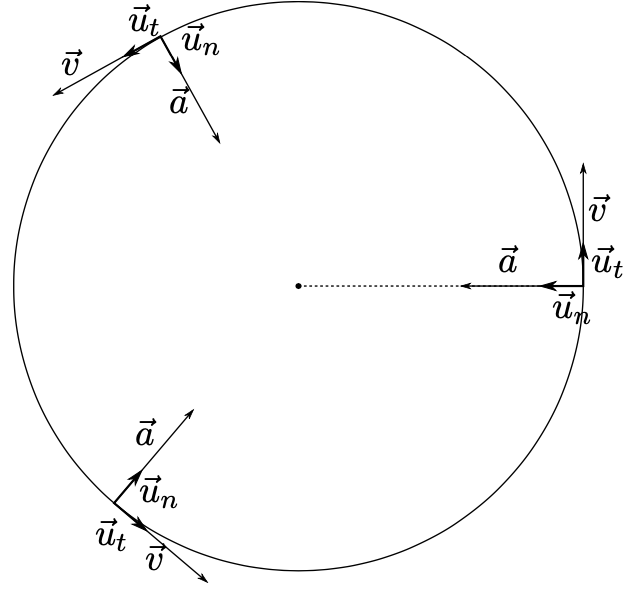
\includegraphics[scale=.5]{figures/cinematique_5}
\blocgris{MCU}{
Dans un MRU, les coordonnées du vecteur accélération s'écrivent simplement:
$$ \overrightarrow{a(t)}=\frac{v^2}{R} .\vec{u_n}$$ 

	 \[
 \overrightarrow{a(t)} 
\begin{pmatrix}
	a_t(t) = \trou{ 0  } \\
		a_n(t) = \frac{v^2}{R} = cste
\end{pmatrix}
\]
}

\newpage
\section{Deuxième Synthèse des résultats}
\etiquette{Cas des mouvements circulaires}


\begin{tabular}{|l|l|l|l|}
\hline

  Mouvements&Description & Mathématiques & Exemples\\
\hline  \hline
MCU & valeur de vitesse constante& $v=cste$& - disque vinyl sur platine\\
    & $\vec{v(t)}$ tourne& $\vec{v(t)}\neq \overrightarrow{cste}$ & -Terre autour du Soleil\\
    & $\vec{a(t)}$ centripète, tourne & $\vec{a}\neq\overrightarrow{cste}$&\\
    & accélération constante&$a=\frac{v^2}{R}=cste$& \\
    \hline
    MC général& -vitesse tangente au cercle& $\vec{v(t)}=v(t).\vec{u_t}$ & -Roue de voiture au\\
    & -vitesse non constante& $v(t)\neq 0$& démarrage\\
    &-accélération vers l'intérieur& $\vec{a(t)}=a_t.\vec{u_t}+a_n.\vec{u_n}$ & \\
    & du cercle & $a_t=\frac{dv(t)}{dt}\neq 0$ & \\
    & & $a_n=\frac{v^2(t)}{R}$&\\
    \hline
    
     
\end{tabular}

\etiquette{Réactivation}

Pour chacun des mouvements du tableau précédent: 
\begin{enumerate}
	\item Représenter une chronophotographie du mouvement.
	\item Représenter quelques vecteurs vitesses de manière réaliste.
	\item Représenter quelques vecteurs accélérations de manière réaliste.
\end{enumerate}

\newpage
\includegraphics[scale=.88]{figures/cinematique_7}
